\documentclass[11pt,a4paper]{article}
\usepackage[utf8]{inputenc}
\usepackage[T1]{fontenc}
\usepackage[english]{babel}
\usepackage[margin=2.5cm]{geometry}
\usepackage{booktabs,array,tabularx}
\usepackage{amsmath,amssymb}
\usepackage{xcolor}
\usepackage{listings}
\usepackage{pgfplots}
\usepackage{hyperref}
\usepackage{caption}
\pgfplotsset{compat=1.17}
\hypersetup{colorlinks=true,linkcolor=blue!50!black,urlcolor=blue!50!black}

\lstset{
  language=C++, basicstyle=\ttfamily\footnotesize, keywordstyle=\color{blue!60!black},
  commentstyle=\color{green!40!black}, numbers=left, numberstyle=\tiny, breaklines=true,
  frame=single, columns=fullflexible, keepspaces=true, showstringspaces=false
}

\title{Practical Work 1 -- ``Making Change'':\\ Greedy, Exhaustive Enumeration and Pruned Search}
\author{Oumnia Chiouikh \and Malick Diop}
\date{}

\begin{document}
\maketitle

\begin{center}
UE 7 -- Mobility in Smart Cities \quad Dynamic Transportation \& Exact Solving (Ph.\ Canalda)\\
Code repository: \url{https://github.com/<your-account>/<your-repository>} % TODO
\end{center}

\tableofcontents
\newpage

%------------------------------------------------------------
\section{Objectives}
This practical work studies one small combinatorial problem, \emph{making change}, to compare three ways of solving it exactly: a \textbf{greedy} method, \textbf{exhaustive enumeration} of all solutions, and a \textbf{recursive search with cuts} (branch and bound). The instance given in the course is the coin list $L=\{5, 2, 1, 0.5, 0.2, 0.1, 0.05\}$~\texteuro{} and the amount $m=12.35$~\texteuro.

Following the ``challenge'' slide of the course, each method is evaluated on: execution time, printed output (screen memory), dynamic memory used to keep the best solution, memory shared between recursive calls, and number of cuts.

%------------------------------------------------------------
\section{Team and organisation}
\begin{center}
\begin{tabular}{@{}ll@{}}
\toprule
Member & Contribution \\
\midrule
Oumnia Chiouikh & [TODO: e.g.\ greedy and exhaustive programs] \\
Malick Diop & [TODO: e.g.\ cut versions, measurements] \\
\bottomrule
\end{tabular}
\end{center}
Language: C++17, compiled with \texttt{g++ -O2 -std=c++17}.

%------------------------------------------------------------
\section{Design}
\subsection{Data representation}
All amounts are \textbf{integers in cents} ($L=\{500,200,100,50,20,10,5\}$, $m=1235$). This avoids floating-point errors such as the \texttt{-0.0} remainder visible in one student output of the course, and makes \texttt{\%} and \texttt{/} exact.

\subsection{A solution}
A solution is an array $S$ of the same length as $L$, where $S[k]$ is the number of coins of value $L[k]$. Its cost is the total number of coins $\sum_k S[k]$. It is valid when $\sum_k S[k]\cdot L[k]=m$.

\subsection{Programs and mapping to the assignment}
\begin{center}
\begin{tabularx}{\textwidth}{@{}lXl@{}}
\toprule
File & Method & Assignment item \\
\midrule
\texttt{greedy.cpp} & Greedy, iterative & Prg1 \\
\texttt{allsolutions.cpp} & Recursive enumeration of all solutions, ascending counts, no cut; prints the first 10 solutions and counts the rest & Prg2 / Prg3 \\
\texttt{rwc.cpp} & Recursive search, incumbent best solution, two cuts, counts tried in ascending order ($0,1,2,\dots$) & Prg4 / Prg5 / Prg6 \\
\texttt{sib.cpp} & Same cuts, counts tried in \textbf{descending} order (largest first) & Prg6 bis \\
\bottomrule
\end{tabularx}
\end{center}

\subsection{Algorithms}
\paragraph{Greedy.} For each coin from largest to smallest: take \texttt{remaining / coin} coins, then \texttt{remaining \%= coin}. Complexity $O(n)$ for $n$ coin types.

\paragraph{Enumeration.} \texttt{solve(i, remaining, S)}: if \texttt{remaining == 0} a solution is found; if $i$ is past the last coin the branch is a dead end; otherwise try $j=0\dots \lfloor \texttt{remaining}/L[i]\rfloor$ coins of type $i$, recurse on $i+1$, and reset $S[i]$ to $0$ when coming back (backtracking). The only data structure is one array $S$ passed by reference.

\paragraph{Cuts.} Two cuts are added to the enumeration:
\begin{itemize}
  \item \emph{Cut 1:} if \texttt{used >= best}, the branch cannot improve the incumbent.
  \item \emph{Cut 2 (optimistic bound):} with the largest remaining coin $L[i]$, at least $\lceil \texttt{remaining}/L[i]\rceil$ more coins are needed; if $\texttt{used}+\lceil \texttt{remaining}/L[i]\rceil \ge \texttt{best}$, stop.
\end{itemize}
\texttt{rwc.cpp} tries $j=0,1,2,\dots$ and \texttt{sib.cpp} tries $j=\max,\dots,1,0$. Only the order differs, so any difference in effort comes from how early a good incumbent is found.

%------------------------------------------------------------
\section{Tests and results}
Measurements were made on the target instance ($m=1235$). Counters (calls, cuts, improvements) come from an instrumented copy of the same logic (\texttt{bench.cpp}); times are averages over repeated runs on one machine (\texttt{-O2}), so they are indicative and the ratios matter more than absolute values. % TODO: rerun on your machine

\subsection{Result on the course example}
\begin{center}
\begin{tabularx}{\textwidth}{@{}lX@{}}
\toprule
Method & Result \\
\midrule
Greedy & $2\times5 + 1\times2 + 1\times0.20 + 1\times0.10 + 1\times0.05$~\texteuro{} = \textbf{6 coins} \\
Exhaustive & \textbf{266\,724} valid solutions, from 6 coins (best) to 247 coins ($247\times0.05$~\texteuro) \\
\texttt{rwc} (cut, ascending) & best = \textbf{6 coins} (same solution) \\
\texttt{sib} (cut, descending) & best = \textbf{6 coins} (same solution) \\
\bottomrule
\end{tabularx}
\end{center}
The total of 266\,724 was checked independently with a classical coin-change counting table (dynamic programming).

\subsection{Challenge table ($m=12.35$~\texteuro)}
\begin{center}
\footnotesize
\begin{tabularx}{\textwidth}{@{}>{\raggedright\arraybackslash}p{2.6cm}>{\raggedright\arraybackslash}X>{\raggedright\arraybackslash}X>{\raggedright\arraybackslash}X>{\raggedright\arraybackslash}X@{}}
\toprule
Criterion & Greedy & Exhaustive & Cut, ascending (\texttt{rwc}) & Cut, descending (\texttt{sib}) \\
\midrule
Recursive calls & -- (7 loop steps) & 12\,607\,231 & 20\,936 & \textbf{22} \\
Execution time & $\approx$ 14 ns & $\approx$ 44 ms (no printing) & $\approx$ 0.07 ms & $\approx$ 0.0001 ms (timer limit) \\
Solutions / improvements & 1 & 266\,724 & 242 improvements & 1 improvement \\
Cuts & -- & 0 & 4\,731 & 10 \\
Dead-end branches & -- & 12\,063\,270 & 15\,494 & 1 \\
Printed output (full run) & 10 lines, 209 bytes & 266\,724 lines, $\approx$ 8.4 MB if all printed to a file (submitted program prints 10 and counts) & 503 lines, 9\,067 bytes & 16 lines, 591 bytes (with scaling table) \\
Memory for best solution & 7-int result & none kept (counted only) & 1 array of 7 ints (28 B), overwritten 242 times & no array kept; improving solution printed \\
Memory shared by calls & -- & 1 array $S$ (28 B) shared by all frames & $S$, \texttt{bestSolution}, \texttt{best} shared by reference & $S$ and global \texttt{best} shared \\
\bottomrule
\end{tabularx}
\end{center}
``Shared memory'' means the recursion never copies the solution: one array of 7 integers is shared by all 8 levels (maximum depth = number of coin types + 1) instead of one copy per level.

\subsection{Growth with the amount}
\begin{table}[h!]
\centering
\small
\begin{tabular}{@{}rrrrrrr@{}}
\toprule
Amount (cents) & \multicolumn{2}{c}{Exhaustive} & \multicolumn{2}{c}{Cut ascending} & \multicolumn{2}{c}{Cut descending} \\
\cmidrule(lr){2-3}\cmidrule(lr){4-5}\cmidrule(l){6-7}
 & calls & time (ms) & calls & cuts & calls & cuts \\
\midrule
200  & 3\,572 & 0.021 & 610 & 109 & 4 & 1 \\
400  & 53\,392 & 0.223 & 2\,270 & 469 & 5 & 2 \\
600  & 327\,663 & 1.086 & 4\,984 & 1\,080 & 6 & 2 \\
800  & 1\,314\,431 & 4.242 & 8\,745 & 1\,941 & 7 & 3 \\
1000 & 4\,099\,986 & 12.675 & 13\,557 & 3\,052 & 4 & 2 \\
1200 & 10\,788\,424 & 32.927 & 19\,423 & 4\,415 & 6 & 3 \\
1400 & 25\,081\,194 & 72.324 & 26\,335 & 6\,027 & 7 & 4 \\
1600 & 53\,045\,505 & 158.355 & 34\,301 & 7\,890 & 8 & 4 \\
\bottomrule
\end{tabular}
\caption{Work as a function of the amount (7 euro coins).}
\end{table}

\begin{figure}[h!]
\centering
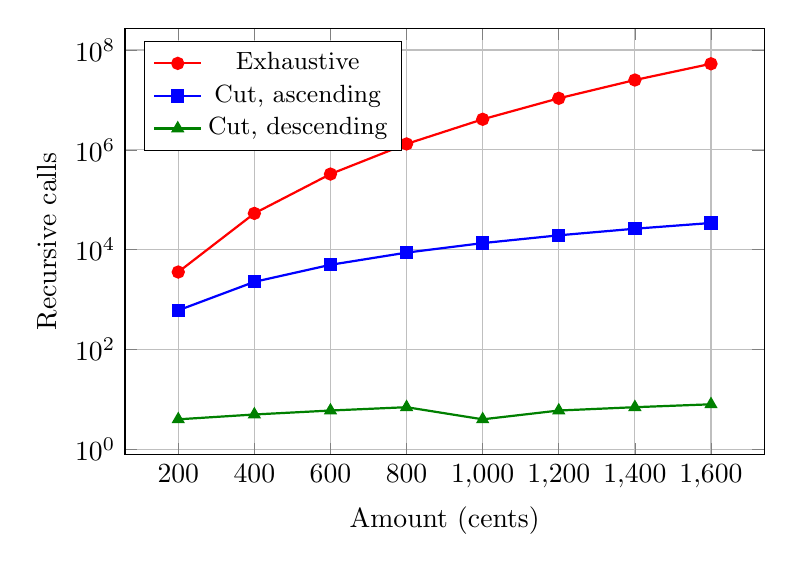
\begin{tikzpicture}
\begin{axis}[width=0.8\textwidth,height=7cm,xlabel={Amount (cents)},ylabel={Recursive calls},
  ymode=log,legend pos=north west,grid=both,legend style={font=\small}]
\addplot[mark=*,thick,red] coordinates {(200,3572)(400,53392)(600,327663)(800,1314431)(1000,4099986)(1200,10788424)(1400,25081194)(1600,53045505)};
\addlegendentry{Exhaustive}
\addplot[mark=square*,thick,blue] coordinates {(200,610)(400,2270)(600,4984)(800,8745)(1000,13557)(1200,19423)(1400,26335)(1600,34301)};
\addlegendentry{Cut, ascending}
\addplot[mark=triangle*,thick,green!50!black] coordinates {(200,4)(400,5)(600,6)(800,7)(1000,4)(1200,6)(1400,7)(1600,8)};
\addlegendentry{Cut, descending}
\end{axis}
\end{tikzpicture}
\caption{Recursive calls versus amount (logarithmic scale).}
\end{figure}

%------------------------------------------------------------
\section{Evaluation and analysis}
\subsection{Greedy}
The greedy method is by far the cheapest (7 divisions, no recursion, constant memory) and gives the optimum here. This is not luck: the euro system is a \textbf{canonical} coin system, where the best local choice (largest coin first) is also the best global choice. The method is exact only under this condition. Two counter-examples from the course material:
\begin{itemize}
  \item $L=\{5,2,1.5\}$, $m=9.5$. In units of 0.5~\texteuro{} this is $\{10,4,3\}$ and $m=19$. Greedy takes $10+4+4=18$ and is stuck with remainder 1: it announces ``impossible'', although $10+3+3+3=19$ exists (4 coins).
  \item $L=\{3,2\}$, $m=7$. Greedy takes $2\times3=6$, remainder 1, and fails. Exhaustive search tries $j=0,1,2$ coins of value 3 and finds the only solution $1\times3+2\times2$ (3 coins).
\end{itemize}
Hence the need for exhaustive and pruned versions when the coin system is not canonical, or when constraints are added (limited number of coins, unordered list).

\subsection{Exhaustive enumeration}
The exhaustive search is exact and generic, but its cost explodes: 12.6 million calls and 266\,724 solutions for 12.35~\texteuro, about 53 million calls for 16~\texteuro. Between 800 and 1600 cents the calls are multiplied by about 40, i.e.\ a polynomial of degree about 5 to 6 in the amount (the number of solutions grows like $m^{n-1}$ for $n$ coin types). Most of the work is wasted: 12\,063\,270 of the 12\,607\,231 calls are dead ends reaching the end of the coin list with a non-zero remainder.

Printing is the other cost: printing all 266\,724 solutions produces about 8.4~MB, while counting avoids it. The recursion itself needs almost no memory (one array of 28 bytes), but I/O through buffers is slow.

\subsection{Cuts (branch and bound)}
\begin{itemize}
  \item \textbf{Ascending order} (\texttt{rwc}): the search first finds the worst solutions (247, 246, 245\dots{} coins), so the incumbent improves 242 times before reaching 6. Even so, the cuts reduce the work from 12.6 million to 20\,936 calls ($\approx 600\times$ fewer).
  \item \textbf{Descending order} (\texttt{sib}): the first complete branch is the greedy one (6 coins). The incumbent is optimal from the first leaf and Cut~2 removes everything else: \textbf{22 calls, 10 cuts}, i.e.\ $\approx 570\,000\times$ fewer calls than exhaustive and $\approx 950\times$ fewer than the ascending cut. This answers Prg6~bis: \emph{the order matters more than the cut itself}, because an early good incumbent makes the bound effective.
  \item On the scaling table, the descending version needs only 4 to 8 calls whatever the amount, while the ascending version still grows (610 to 34\,301 calls).
\end{itemize}

\paragraph{Observation on Cut 1.} In both programs Cut~1 never fires (0 times). This is not a coincidence: a child is called with $\texttt{used}+j$ where $j\le\lfloor r/L[i]\rfloor\le\lceil r/L[i]\rceil$, and the parent has already checked $\texttt{used}+\lceil r/L[i]\rceil<\texttt{best}$. So Cut~1 is implied by Cut~2 except at the root and could be removed without changing the result. All cuts counted are Cut~2.

\subsection{Limits and possible improvements}
\begin{itemize}
  \item The descending order works so well here because the euro system is canonical, so the greedy path is optimal. On a non-canonical system the first incumbent can be poor and the gain smaller (to test on $\{10,4,3\}$, $m=19$).
  \item The bound $\lceil r/L[i]\rceil$ is simple; a bound using the next coins, or a table of optimal counts for small amounts (dynamic programming, $O(n\cdot m)$), would cut more.
  \item \texttt{sib.cpp} prints the improving solution but does not keep it in an array, whereas Prg5 asks for a stored best solution; \texttt{rwc.cpp} keeps it (\texttt{bestSolution}).
  \item Times come from one machine and the timer is too coarse for the 22-call run; use larger amounts or repeated runs.
\end{itemize}

%------------------------------------------------------------
\section{Link with the mini-project}
The same ideas apply to the mobility problems of the course: enumerating all routes or meeting points is exact but exponential; keeping the best cost found so far and abandoning any partial route whose optimistic cost already exceeds it is the same pruning as Cut~2; exploring the most promising choices first is the same principle as a good heuristic ordering. Greedy is the fast baseline and the exact search validates it.

%------------------------------------------------------------
\section{How to reproduce}
\begin{lstlisting}[language=bash,numbers=none]
g++ -O2 -std=c++17 -o greedy greedy.cpp
g++ -O2 -std=c++17 -o allsolutions allsolutions.cpp
g++ -O2 -std=c++17 -o rwc rwc.cpp
g++ -O2 -std=c++17 -o sib sib.cpp
./greedy
./allsolutions > all_output.txt
./rwc > rwc_output.txt ; wc -l rwc_output.txt
./sib > sib_output.txt
\end{lstlisting}
The assignment also asks for the class diagram, a \texttt{CORRECT\_} result file compared with \texttt{diff}, and the Prg2~bis / Prg3 variants (reverse-order enumeration without cut, solutions stored in a 2D array). These are not covered by the four programs submitted here. % TODO: add before 30 November 2026

%------------------------------------------------------------
\section{Conclusion}
For the euro system all three approaches agree on the optimum of 6 coins for 12.35~\texteuro. Greedy is the fastest but only guaranteed for canonical systems; exhaustive search is general but needs 12.6 million calls; pruned search with the largest counts first keeps the generality of exhaustive search at almost the cost of greedy (22 calls). Exact methods need pruning, and the exploration order can matter more than the pruning rule.

\appendix
\section{Source code}
\subsection{greedy.cpp}
\begin{lstlisting}
#include <iostream>
#include <vector>
#include <iomanip>

using namespace std;

int main() {

    // List of available coins, ordered from largest to smallest
    vector<int> coins = {500, 200, 100, 50, 20, 10, 5};

    // Amount of change: 12.35 euros = 1235 cents
    int amount = 1235;

    cout << fixed << setprecision(2);
    cout << "Amount to return: " << amount / 100.0 << " euros\n\n";

    int remaining = amount;
    int totalCoins = 0;

    // Greedy algorithm
    for (int coin : coins) {

        // Number of coins of this value
        int number = remaining / coin;

        if (number > 0) {

            cout << number
                 << " coin(s) of "
                 << coin / 100.0
                 << " euros\n";

            totalCoins += number;

            // Calculate the remaining amount
            remaining = remaining % coin;
        }

        // Stop if the whole amount has been returned
        if (remaining == 0) {
            break;
        }
    }

    cout << "\nTotal number of coins: "
         << totalCoins << endl;

    if (remaining != 0) {
        cout << "It is impossible to make the exact change.\n";
    } else {
        cout << "Change successfully calculated.\n";
    }

    return 0;
}
\end{lstlisting}

\subsection{allsolutions.cpp}
\begin{lstlisting}
#include <iostream>
#include <vector>
#include <chrono>
#include <iomanip>

using namespace std;

vector<int> coins = {500, 200, 100, 50, 20, 10, 5};   // in cents
long long nbSolutions = 0;   // number of solutions found
long long nbCalls = 0;       // number of recursive calls (measures the work)
bool verbose = true;         // print the first solutions

// S[k] = number of coins of value coins[k] chosen so far
void solve(int i, int remaining, vector<int>& S) {
    nbCalls++;

    // Stop condition 1: the whole amount is returned -> a solution
    if (remaining == 0) {
        nbSolutions++;
        if (verbose && nbSolutions <= 10) {
            cout << "Solution " << nbSolutions << ": ";
            int total = 0;
            for (size_t k = 0; k < coins.size(); k++) {
                if (S[k] > 0) {
                    cout << S[k] << "x" << coins[k] / 100.0 << "  ";
                    total += S[k];
                }
            }
            cout << "(" << total << " coins)\n";
        }
        return;
    }

    // Stop condition 2: no more coin types -> no solution on this branch
    if (i >= (int)coins.size()) return;

    // Try every possible number of coins of type i: 0 .. remaining / coins[i]
    for (int j = 0; j <= remaining / coins[i]; j++) {
        S[i] = j;
        solve(i + 1, remaining - j * coins[i], S);
    }
    S[i] = 0;   // undo before going back up
}

int main() {
    int amount = 1235;   // 12.35 euros
    vector<int> S(coins.size(), 0);

    cout << "Amount: " << amount / 100.0 << " euros\n\n";
    solve(0, amount, S);
    cout << "\nTotal number of solutions: " << nbSolutions << "\n";
    cout << "Recursive calls: " << nbCalls << "\n\n";

    // Table for the complexity curve
    verbose = false;
    cout << "amount(cents)  solutions      calls        time(ms)\n";
    for (int a = 200; a <= 1600; a += 200) {
        nbSolutions = 0;
        nbCalls = 0;
        fill(S.begin(), S.end(), 0);
        auto t0 = chrono::steady_clock::now();
        solve(0, a, S);
        auto t1 = chrono::steady_clock::now();
        double ms = chrono::duration<double, milli>(t1 - t0).count();
        cout << setw(10) << a << setw(12) << nbSolutions
             << setw(12) << nbCalls << setw(14) << fixed
             << setprecision(3) << ms << "\n";
    }
    return 0;
}
\end{lstlisting}

\subsection{rwc.cpp}
\begin{lstlisting}
#include <iostream>
#include <vector>
#include <iomanip>
#include <climits>
#include <algorithm>

using namespace std;

// ------------------------------------------------------------
// Display a solution
// ------------------------------------------------------------
void displaySolution(const vector<int>& coins,
                     const vector<int>& solution,
                     int totalCoins)
{
    cout << "\nBest solution found:\n";

    for (int i = 0; i < (int)coins.size(); i++)
    {
        if (solution[i] > 0)
        {
            cout << solution[i]
                 << " coin(s) of "
                 << fixed << setprecision(2)
                 << coins[i] / 100.0
                 << " euros\n";
        }
    }

    cout << "Total number of coins: "
         << totalCoins << endl;
}


// ------------------------------------------------------------
// Recursive algorithm with cuts
// ------------------------------------------------------------
void recursiveWithCut(
    const vector<int>& coins,
    int index,
    int remaining,
    vector<int>& currentSolution,
    int currentNumberOfCoins,
    int& bestNumberOfCoins,
    vector<int>& bestSolution)
{
    // --------------------------------------------------------
    // STOP CONDITION 1:
    // Exact amount has been reached.
    // --------------------------------------------------------
    if (remaining == 0)
    {
        // We found a better solution
        if (currentNumberOfCoins < bestNumberOfCoins)
        {
            bestNumberOfCoins = currentNumberOfCoins;
            bestSolution = currentSolution;

            cout << "\nImproved solution found: "
                 << bestNumberOfCoins
                 << " coins\n";
        }

        return;
    }

    // --------------------------------------------------------
    // STOP CONDITION 2:
    // We have used all coin types.
    // --------------------------------------------------------
    if (index >= (int)coins.size())
    {
        return;
    }

    // --------------------------------------------------------
    // CUT 1:
    //
    // If the current solution already uses as many coins
    // as the best solution, continuing cannot improve it.
    // --------------------------------------------------------
    if (currentNumberOfCoins >= bestNumberOfCoins)
    {
        return;
    }

    // --------------------------------------------------------
    // CUT 2:
    //
    // Calculate an optimistic lower bound.
    //
    // The largest remaining coin is coins[index].
    // Even in the best possible case, we need at least:
    //
    // ceil(remaining / coins[index])
    //
    // additional coins.
    // --------------------------------------------------------
    int minimumAdditionalCoins =
        (remaining + coins[index] - 1) / coins[index];

    if (currentNumberOfCoins + minimumAdditionalCoins
        >= bestNumberOfCoins)
    {
        return;
    }

    // --------------------------------------------------------
    // Try all possible numbers of coins of coins[index].
    //
    // j = 0, 1, 2, ..., maximum possible number
    // --------------------------------------------------------
    int maximumNumber =
        remaining / coins[index];

    for (int j = 0; j <= maximumNumber; j++)
    {
        // Add j coins of the current denomination
        currentSolution[index] = j;

        // Calculate the new remaining amount
        int newRemaining =
            remaining - j * coins[index];

        // Recursive call with the next denomination
        recursiveWithCut(
            coins,
            index + 1,
            newRemaining,
            currentSolution,
            currentNumberOfCoins + j,
            bestNumberOfCoins,
            bestSolution
        );

        // Remove the choice before trying the next one
        currentSolution[index] = 0;
    }
}


// ------------------------------------------------------------
// Main
// ------------------------------------------------------------
int main()
{
    // Coins in decreasing order
    // Values are expressed in cents
    vector<int> coins =
    {
        500,  // 5.00 EUR
        200,  // 2.00 EUR
        100,  // 1.00 EUR
        50,   // 0.50 EUR
        20,   // 0.20 EUR
        10,   // 0.10 EUR
        5     // 0.05 EUR
    };

    // 12.35 EUR = 1235 cents
    int amount = 1235;

    // Current candidate solution
    vector<int> currentSolution(coins.size(), 0);

    // Best solution found so far
    vector<int> bestSolution(coins.size(), 0);

    // Start with infinity
    int bestNumberOfCoins = INT_MAX;

    cout << fixed << setprecision(2);

    cout << "========================================\n";
    cout << "   MAKES CHANGE - RECURSIVE WITH CUT\n";
    cout << "========================================\n\n";

    cout << "Amount: "
         << amount / 100.0
         << " euros\n\n";

    cout << "Searching for the best solution...\n";

    // Start recursive search
    recursiveWithCut(
        coins,
        0,                  // Start with first coin
        amount,             // Remaining amount
        currentSolution,    // Current solution
        0,                  // Number of coins currently used
        bestNumberOfCoins,  // Best number found
        bestSolution        // Best combination
    );

    // --------------------------------------------------------
    // Display final result
    // --------------------------------------------------------
    cout << "\n========================================\n";
    cout << "              FINAL RESULT\n";
    cout << "========================================\n";

    if (bestNumberOfCoins == INT_MAX)
    {
        cout << "No exact solution exists.\n";
    }
    else
    {
        displaySolution(
            coins,
            bestSolution,
            bestNumberOfCoins
        );
    }

    return 0;
}
\end{lstlisting}

\subsection{sib.cpp}
\begin{lstlisting}
#include <iostream>
#include <vector>
#include <chrono>
#include <iomanip>
#include <climits>

using namespace std;

vector<int> coins = {500, 200, 100, 50, 20, 10, 5};   // in cents, descending
int best = INT_MAX;          // fewest coins found so far
long long nbCalls = 0;       // number of recursive calls
bool verbose = true;

// S[k] = number of coins of value coins[k]; used = coins chosen so far
void solve(int i, int remaining, int used, vector<int>& S) {
    nbCalls++;

    // CUT 1: already as many coins as the best solution -> cannot improve
    if (used >= best) return;

    // Stop condition: amount fully returned -> it improves the best
    if (remaining == 0) {
        best = used;
        if (verbose) {
            cout << "Improving solution (" << used << " coins): ";
            for (size_t k = 0; k < coins.size(); k++)
                if (S[k] > 0) cout << S[k] << "x" << coins[k] / 100.0 << "  ";
            cout << "\n";
        }
        return;
    }

    // No more coin types -> dead end
    if (i >= (int)coins.size()) return;

    // CUT 2: even with the largest remaining coin, we need at least
    // ceil(remaining / coins[i]) more coins. If that cannot improve, stop.
    int minMore = (remaining + coins[i] - 1) / coins[i];
    if (used + minMore >= best) return;

    // Try the largest counts first: good solutions are found early,
    // so the cuts become effective sooner
    for (int j = remaining / coins[i]; j >= 0; j--) {
        S[i] = j;
        solve(i + 1, remaining - j * coins[i], used + j, S);
    }
    S[i] = 0;   // undo (backtracking)
}

int main() {
    int amount = 1235;   // 12.35 euros
    vector<int> S(coins.size(), 0);

    cout << "Amount: " << amount / 100.0 << " euros\n\n";
    solve(0, amount, 0, S);
    cout << "\nBest number of coins: " << best << "\n";
    cout << "Recursive calls: " << nbCalls << "\n\n";

    // Table to compare with the version without cut
    verbose = false;
    cout << "amount(cents)  best coins      calls        time(ms)\n";
    for (int a = 200; a <= 1600; a += 200) {
        best = INT_MAX;
        nbCalls = 0;
        fill(S.begin(), S.end(), 0);
        auto t0 = chrono::steady_clock::now();
        solve(0, a, 0, S);
        auto t1 = chrono::steady_clock::now();
        double ms = chrono::duration<double, milli>(t1 - t0).count();
        cout << setw(10) << a << setw(12) << best
             << setw(14) << nbCalls << setw(14) << fixed
             << setprecision(3) << ms << "\n";
    }
    return 0;
}
\end{lstlisting}

\subsection{bench.cpp (measurement harness)}
\begin{lstlisting}
// Measurement harness: same logic as allsolutions/rwc/sib, with extra counters (cuts, improvements)
#include <bits/stdc++.h>
using namespace std;
vector<int> coins={500,200,100,50,20,10,5};
long long calls,cut1,cut2,impr,sols,deadends; int best; bool desc; size_t maxDepth,depth;
void enumAll(int i,int rem,vector<int>&S,ostream*out){
  calls++; if(rem==0){sols++; if(out){for(size_t k=0;k<coins.size();k++) if(S[k]) *out<<S[k]<<"x"<<coins[k]/100.0<<" "; *out<<"\n";} return;}
  if(i>=(int)coins.size()){deadends++;return;}
  for(int j=0;j<=rem/coins[i];j++){S[i]=j;enumAll(i+1,rem-j*coins[i],S,out);} S[i]=0;}
// rwc logic (asc) / sib logic (desc); rwc checks rem==0 BEFORE cut1, sib AFTER
void cut(int i,int rem,int used,vector<int>&S,bool rwcOrder){
  calls++;
  if(rwcOrder){
    if(rem==0){ if(used<best){best=used;impr++;} return;}
    if(i>=(int)coins.size()){deadends++;return;}
    if(used>=best){cut1++;return;}
  } else {
    if(used>=best){cut1++;return;}
    if(rem==0){best=used;impr++;return;}
    if(i>=(int)coins.size()){deadends++;return;}
  }
  int mn=(rem+coins[i]-1)/coins[i];
  if(used+mn>=best){cut2++;return;}
  if(desc){for(int j=rem/coins[i];j>=0;j--){S[i]=j;cut(i+1,rem-j*coins[i],used+j,S,rwcOrder);}}
  else {for(int j=0;j<=rem/coins[i];j++){S[i]=j;cut(i+1,rem-j*coins[i],used+j,S,rwcOrder);}}
  S[i]=0;}
template<class F> double timeit(F f,int rep){auto t0=chrono::steady_clock::now();for(int r=0;r<rep;r++)f();auto t1=chrono::steady_clock::now();return chrono::duration<double,milli>(t1-t0).count()/rep;}
int main(){
  int m=1235; vector<int>S(7,0);
  {calls=sols=deadends=0; ofstream o("AllTheSolutionsTest1.txt"); enumAll(0,m,S,&o); o.close();
   printf("ALL(print to file): calls=%lld sols=%lld deadends=%lld\n",calls,sols,deadends);}
  double t=timeit([&]{calls=sols=deadends=0;fill(S.begin(),S.end(),0);enumAll(0,m,S,nullptr);},20);
  printf("ALL(no print) time=%.3f ms calls=%lld\n",t,calls);
  for(int mode=0;mode<2;mode++){ // 0 = rwc (asc), 1 = sib (desc)
    desc=mode; 
    auto run=[&]{calls=cut1=cut2=impr=deadends=0;best=INT_MAX;fill(S.begin(),S.end(),0);cut(0,m,0,S,mode==0);};
    double tt=timeit(run,200); run();
    printf("%s: best=%d calls=%lld cut1=%lld cut2=%lld cuts=%lld improvements=%lld deadends=%lld time=%.4f ms\n",mode?"SIB(desc)":"RWC(asc)",best,calls,cut1,cut2,cut1+cut2,impr,deadends,tt);
  }
  // greedy time
  vector<int> c=coins; double tg=timeit([&]{int r=m,n=0;volatile int tot=0;for(int x:c){n=r/x;tot+=n;r%=x;}},1000000);
  printf("greedy time=%.8f ms (%.1f ns)\n",tg,tg*1e6);
  // scaling table for report
  printf("\namount asc_calls asc_cuts desc_calls desc_cuts all_calls\n");
  for(int a=200;a<=1600;a+=200){
    desc=false;calls=cut1=cut2=0;best=INT_MAX;fill(S.begin(),S.end(),0);cut(0,a,0,S,true);long long c1=calls,k1=cut1+cut2;
    desc=true;calls=cut1=cut2=0;best=INT_MAX;fill(S.begin(),S.end(),0);cut(0,a,0,S,false);long long c2=calls,k2=cut1+cut2;
    calls=sols=deadends=0;fill(S.begin(),S.end(),0);enumAll(0,a,S,nullptr);
    printf("%d %lld %lld %lld %lld %lld\n",a,c1,k1,c2,k2,calls);}
}
\end{lstlisting}


\end{document}
